\documentclass[12pt,fleqn]{article}\usepackage{../../common}
\begin{document}
Hesapsal Sıvı Dinamiği (Computational Fluid Dynamics -CFD-) - 2

Diffusion (Yayınım) Denklemi

Tek boyuttaki yayınım denklemi,

$$
\frac{\partial u}{\partial t} = \nu \frac{\partial^2 u}{\partial x^2}
$$

Dikkat edersek bu denklemde bir ikinci kısmı türev var. Denklemin o
kısmını Merkezi Farklar yaklaşımı ile ayrıksal hale getireceğiz, bu
yaklaşım İleri Farklar ve Geriye Farklar yaklaşımlarının birleştirilmesi ile
elde edilir.

Önce Taylor serilerini hatırlarsak, genel tanım

$$
f(x+h) = f(x) + h f'(x) + \frac{h^2}{2} f''(x) + ...
$$

Biz $u_{i+1}$ ve $u_{i-1}$ açılımını Taylor serisi ile yapmak istiyoruz, daha
önce belirttiğimiz gibi bir önceki ve sonraki $x$ değerleri $\Delta x$
uzaklığında, yani bir önceki

$$
u(x-\Delta x) = u(x) - \Delta x f'(x) + \frac{h^2}{2} u''(x) + ...
$$

İşaretin eksi olmasına dikkat, ve sonraki 

$$
u(x+\Delta x) = u(x) + \Delta x f'(x) + \frac{h^2}{2} u''(x) + ...
$$

Şimdi indisleriyle $u$ için ve [1]'deki formuyla yazalım,

$$
u_{i+1} = u_i + \Delta x \frac{\partial u}{\partial x}\bigg|_i +
\frac{\Delta x^2}{2} \frac{\partial ^2 u}{\partial x^2}\bigg|_i +
\frac{\Delta x^3}{3!} \frac{\partial ^3 u}{\partial x^3}\bigg|_i +
O(\Delta x^4)
$$

$$
u_{i-1} = u_i - \Delta x \frac{\partial u}{\partial x}\bigg|_i +
\frac{\Delta x^2}{2} \frac{\partial ^2 u}{\partial x^2}\bigg|_i -
\frac{\Delta x^3}{3!} \frac{\partial ^3 u}{\partial x^3}\bigg|_i +
O(\Delta x^4)
$$

Bir üstteki denklemin ilk hali $u_i = u_{i-1} ... $ ile ama ufak bir yer
değişimi ile görülen biçim elde edilmiş. 

Son iki formülü toplarsak bazı terimlerin ters işaretli olması sebebiyle iptal
olacağını görebiriliz. Ayrıca yaklaşık temsil açısından $O(\Delta x^4)$ ve daha
üstü kuvvetleri yok sayarsak, 

$$
u_{i+1} + u_{i-1} =
2u_i+\Delta x^2 \frac{\partial ^2 u}{\partial x^2}\bigg|_i +
O(\Delta x^4)
$$

$\frac{\partial ^2 u}{\partial x^2}\bigg|_i$ için çözersek ve tekrar düzenlersek,

$$
\frac{\partial ^2 u}{\partial x^2}=\frac{u_{i+1}-2u_{i}+u_{i-1}}{\Delta x^2} + O(\Delta x^2)
$$

$O(\Delta x^2)$ ifadesi $O(\Delta x^4)$ terimi $\Delta x^2$ ile bölününce ortaya çıktı.

Artık 1D yayınım formülünün nihai ayrıksal halini yazabiliriz,

$$
\frac{u_{i}^{n+1}-u_{i}^{n}}{\Delta t} =
\nu\frac{u_{i+1}^{n}-2u_{i}^{n}+u_{i-1}^{n}}{\Delta x^2}
$$

Daha önce olduğu gibi başlangıç koşuları tanımlı ise tek bilinmeyen
$u_{i}^{n+1}$, bu bilinmeyen eşitliğin solunda kalacak şekilde tekrar
düzenlersek,


$$
u_{i}^{n+1} =
u_{i}^{n}+\frac{\nu\Delta t}{\Delta x^2}(u_{i+1}^{n}-2u_{i}^{n}+u_{i-1}^{n})
$$

Üstteki denklem bize çözümü adım adım ilerletmemizi sağlayacak. Ama bir
başlangıç koşuluna ihtiyacımız var, daha önceki favorimize dönebiliriz, şapka
fonksiyonu. $t=2$'de $u=0$, $0.5\le x\le 1$ aralığında ise $u=1$. 

\begin{minted}[fontsize=\footnotesize]{python}
nx = 41
dx = 2 / (nx - 1)
nt = 20 
nu = 0.3 
sigma = .2 
dt = sigma * dx**2 / nu 


u = np.ones(nx)     
u[int(.5 / dx):int(1 / dx + 1)] = 2 

un = np.ones(nx)

for n in range(nt): 
    un = u.copy() 
    for i in range(1, nx - 1):
        u[i] = un[i] + nu * dt / dx**2 * (un[i+1] - 2 * un[i] + un[i-1])
        
plt.plot(np.linspace(0, 2, nx), u);
plt.savefig('compscieng_app45cfd2_01.png')
\end{minted}

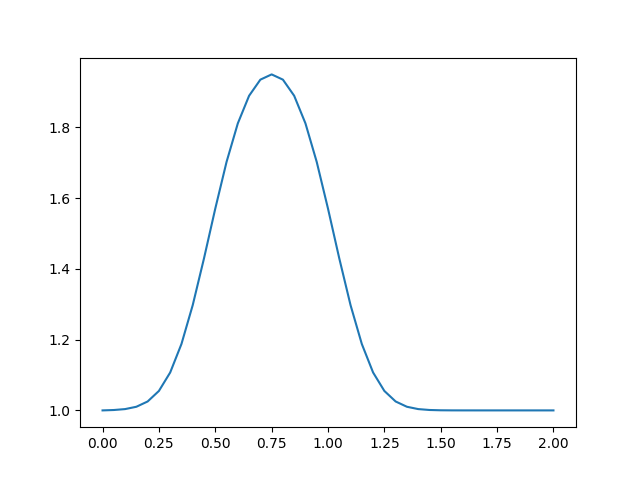
\includegraphics[width=20em]{compscieng_app45cfd2_01.png}

Burger'in Denklemi

Bu denklem tek boyutta suna benziyor

$$
\frac{\partial u}{\partial t} + u \frac{\partial u}{\partial x} =
\nu \frac{\partial ^2u}{\partial x^2}
$$

Goruldugu gibi bu formul gayri lineer taşınım akımı (convection) ile yayinim
(diffusion) formullerinin birlesimi. O zaman denklemi once gordugumuz teknikler
ile ayriksal hale getirebiliriz. 

$$
\frac{u_i^{n+1}-u_i^n}{\Delta t} + u_i^n \frac{u_i^n - u_{i-1}^n}{\Delta x} =
\nu \frac{u_{i+1}^n - 2u_i^n + u_{i-1}^n}{\Delta x^2}
$$

Daha önce olduğu gibi başlangıç koşulumuz var, ona göre denklemi tekrar
düzenliyoruz,

$$
u_i^{n+1} =
u_i^n - u_i^n \frac{\Delta t}{\Delta x} (u_i^n - u_{i-1}^n) +
\nu \frac{\Delta t}{\Delta x^2}(u_{i+1}^n - 2u_i^n + u_{i-1}^n)
$$

Bu örnekte farklı bir başlangıç şartı kullanacağız.

$$
u = -\frac{2 \nu}{\phi} \frac{\partial \phi}{\partial x} + 4 
$$

$$
\phi = \exp \bigg(\frac{-x^2}{4 \nu} \bigg) + \exp \bigg(\frac{-(x-2 \pi)^2}{4 \nu} \bigg)
$$

Bu başlangıç şartlarına göre Burger denkleminin analitik çözümü biliniyor,

$$
u = -\frac{2 \nu}{\phi} \frac{\partial \phi}{\partial x} + 4
$$

$$
\phi = \exp \bigg(\frac{-(x-4t)^2}{4 \nu (t+1)} \bigg) + \exp \bigg(\frac{-(x-4t -2 \pi)^2}{4 \nu(t+1)} \bigg)
$$

Sınır şartı

$$
u(0) = u(2\pi)
$$

Fakat başlangıç şartını belli izgara noktalarında işletebilmek istiyoruz, fakat
üstteki formülde çetrefil bir form var, birşeylerin türevi vs var. Ne yapacağız? 
Paket \verb!sympy! kullanılabilir.

\begin{minted}[fontsize=\footnotesize]{python}
import sympy
from sympy.utilities.lambdify import lambdify
from sympy import init_printing
init_printing(use_latex=True)

x, nu, t = sympy.symbols('x nu t')
phi = (sympy.exp(-(x - 4 * t)**2 / (4 * nu * (t + 1))) +
       sympy.exp(-(x - 4 * t - 2 * sympy.pi)**2 / (4 * nu * (t + 1))))
phiprime = phi.diff(x)

u = -2 * nu * (phiprime / phi) + 4
ufunc = lambdify((t, x, nu), u)
print(ufunc(1, 4, 3))
\end{minted}

\begin{verbatim}
3.49170664206445
\end{verbatim}


\begin{minted}[fontsize=\footnotesize]{python}
nx = 101
nt = 100
dx = 2 * np.pi / (nx - 1)
nu = .07
dt = dx * nu

x = np.linspace(0, 2 * np.pi, nx)
un = np.empty(nx)
t = 0

u = np.asarray([ufunc(t, x0, nu) for x0 in x])
\end{minted}

\begin{minted}[fontsize=\footnotesize]{python}
plt.figure(figsize=(11, 7), dpi=100)
plt.plot(x, u, marker='o', lw=2)
plt.xlim([0, 2 * np.pi])
plt.ylim([0, 10]);
plt.savefig('compscieng_app45cfd2_02.png')
\end{minted}


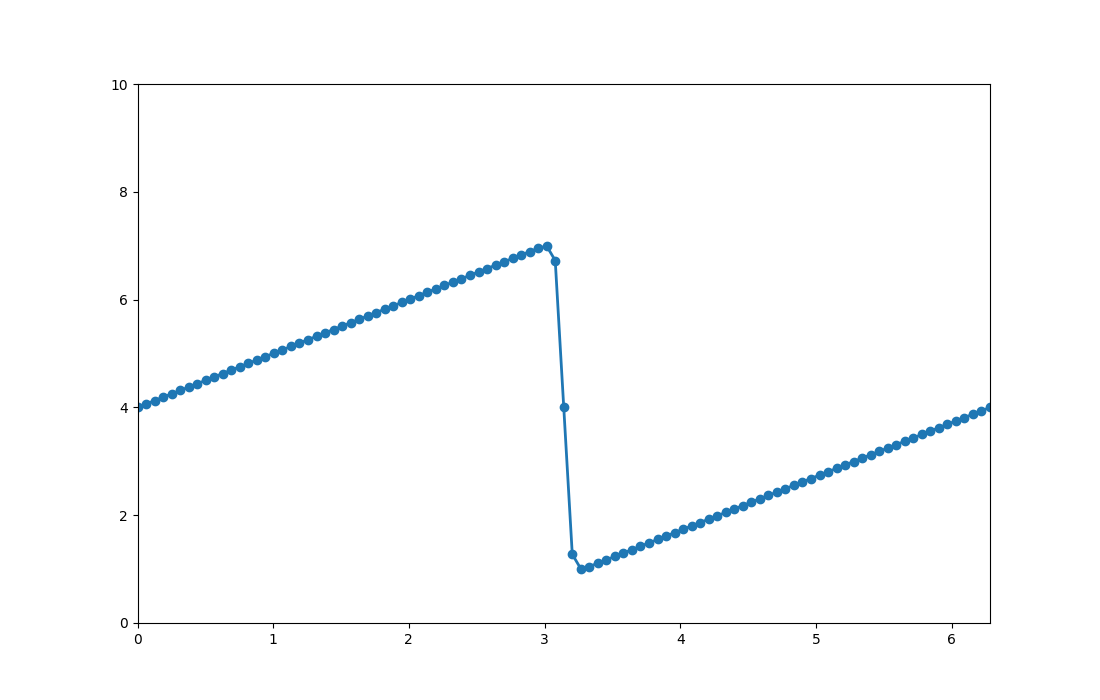
\includegraphics[width=20em]{compscieng_app45cfd2_02.png}

\begin{minted}[fontsize=\footnotesize]{python}
for n in range(nt):
    un = u.copy()
    for i in range(1, nx-1):
        u[i] = un[i] - un[i] * dt / dx *(un[i] - un[i-1]) + nu * dt / dx**2 *\
                (un[i+1] - 2 * un[i] + un[i-1])
    u[0] = un[0] - un[0] * dt / dx * (un[0] - un[-2]) + nu * dt / dx**2 *\
                (un[1] - 2 * un[0] + un[-2])
    u[-1] = u[0]
        
u_analytical = np.asarray([ufunc(nt * dt, xi, nu) for xi in x])
\end{minted}

\begin{minted}[fontsize=\footnotesize]{python}
plt.figure(figsize=(11, 7), dpi=100)
plt.plot(x,u, marker='o', lw=2, label='Computational')
plt.plot(x, u_analytical, label='Analytical')
plt.xlim([0, 2 * np.pi])
plt.ylim([0, 10])
plt.legend();
plt.savefig('compscieng_app45cfd2_03.png')
\end{minted}


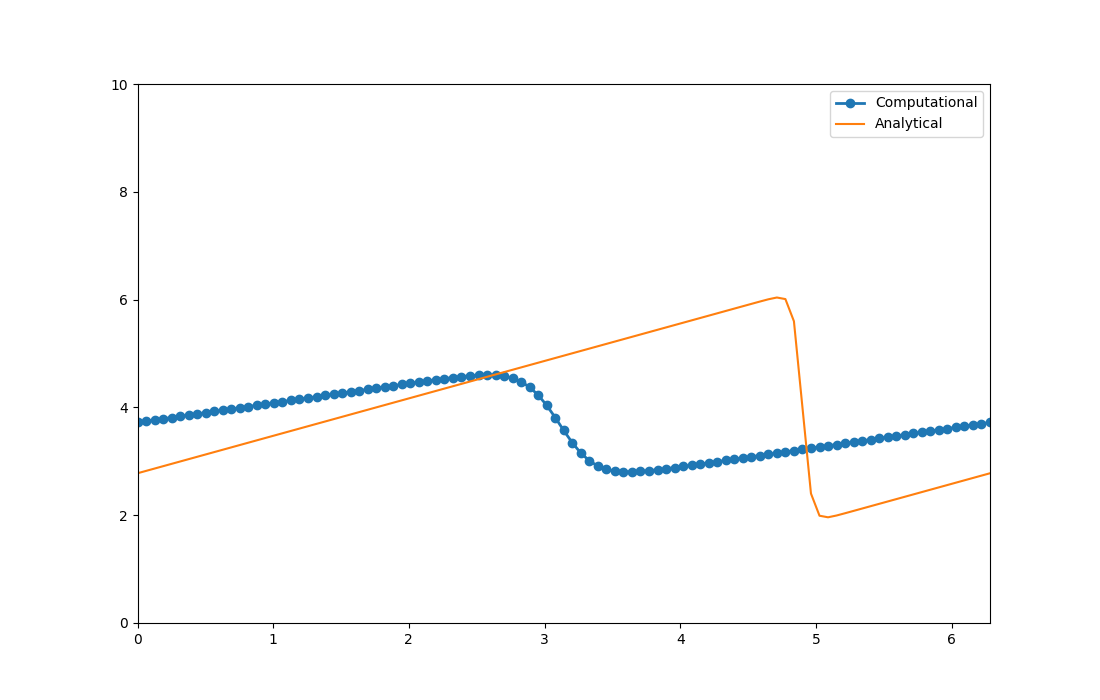
\includegraphics[width=20em]{compscieng_app45cfd2_03.png}







[devam edecek]

Kaynaklar

[1] Barba, {\em 12 steps to Navier–Stokes, Ders 1},
    \url{https://nbviewer.jupyter.org/github/barbagroup/CFDPython/blob/master/lessons/01_Step_1.ipynb}




\end{document}
